%%%%%%%%%%%%%%%%%%%%%%%%%%%%%%%%%%%%%%%%%
% baposter Landscape Poster
% LaTeX Template
% Version 1.0 (11/06/13)
%
% baposter Class Created by:
% Brian Amberg (baposter@brian-amberg.de)
%
% This template has been downloaded from:
% http://www.LaTeXTemplates.com
%
% License:
% CC BY-NC-SA 3.0 (http://creativecommons.org/licenses/by-nc-sa/3.0/)
%
%%%%%%%%%%%%%%%%%%%%%%%%%%%%%%%%%%%%%%%%%

%----------------------------------------------------------------------------------------
%	PACKAGES AND OTHER DOCUMENT CONFIGURATIONS
%----------------------------------------------------------------------------------------

\documentclass[landscape,a0paper,fontscale=0.285]{baposter} % Adjust the font scale/size here

\usepackage{graphicx} % Required for including images
\graphicspath{{figures/}} % Directory in which figures are stored

\usepackage{amsmath} % For typesetting math
\usepackage{amssymb} % Adds new symbols to be used in math mode

\usepackage{booktabs} % Top and bottom rules for tables
\usepackage{enumitem} % Used to reduce itemize/enumerate spacing
\usepackage{palatino} % Use the Palatino font
\usepackage[font=small,labelfont=bf]{caption} % Required for specifying captions to tables and figures

\usepackage{multicol} % Required for multiple columns
\setlength{\columnsep}{1.5em} % Slightly increase the space between columns
\setlength{\columnseprule}{0mm} % No horizontal rule between columns

\usepackage{tikz} % Required for flow chart
\usetikzlibrary{shapes,arrows} % Tikz libraries required for the flow chart in the template

\newcommand{\compresslist}{ % Define a command to reduce spacing within itemize/enumerate environments, this is used right after \begin{itemize} or \begin{enumerate}
\setlength{\itemsep}{1pt}
\setlength{\parskip}{0pt}
\setlength{\parsep}{0pt}
}

\definecolor{lightblue}{rgb}{0.145,0.6666,1} % Defines the color used for content box headers

\begin{document}

\begin{poster}
{
headerborder=closed, % Adds a border around the header of content boxes
colspacing=1em, % Column spacing
bgColorOne=white, % Background color for the gradient on the left side of the poster
bgColorTwo=white, % Background color for the gradient on the right side of the poster
borderColor=lightblue, % Border color
headerColorOne=black, % Background color for the header in the content boxes (left side)
headerColorTwo=lightblue, % Background color for the header in the content boxes (right side)
headerFontColor=white, % Text color for the header text in the content boxes
boxColorOne=white, % Background color of the content boxes
textborder=roundedleft, % Format of the border around content boxes, can be: none, bars, coils, triangles, rectangle, rounded, roundedsmall, roundedright or faded
eyecatcher=true, % Set to false for ignoring the left logo in the title and move the title left
headerheight=0.1\textheight, % Height of the header
headershape=roundedright, % Specify the rounded corner in the content box headers, can be: rectangle, small-rounded, roundedright, roundedleft or rounded
headerfont=\Large\bf\textsc, % Large, bold and sans serif font in the headers of content boxes
%textfont={\setlength{\parindent}{1.5em}}, % Uncomment for paragraph indentation
linewidth=2pt % Width of the border lines around content boxes
}
%----------------------------------------------------------------------------------------
%	TITLE SECTION 
%----------------------------------------------------------------------------------------
%
{
\includegraphics[height=4em]{logo_16_9.png}} % First university/lab logo on the left
{\bf\textsc{Executive Summary}\vspace{0.5em}} % Poster title
{\textsc{\{ Romain Boyre \} \hspace{12pt} Product Owner}} % Author names and institution
{
\includegraphics[height=4em]{logo_16_9.png}} % Second university/lab logo on the right

%----------------------------------------------------------------------------------------
%	OBJECTIFS
%----------------------------------------------------------------------------------------

\headerbox{Objectifs}{name=objectives,column=0,row=0}{

Donner une disruption au web shopping peut avoir des conséquences variées. Nul n’est à l’abri d’une erreur. Pour éviter tout risque, nous brandissons une gamme d’action. Un panel bien vu dans les cas s’agissant de :

\begin{enumerate}\compresslist
\item Placer la cliente au centre du concept
\item Adapter au cours de La conception
\item Limiter l’empreinte carbone 
\item Approfondir la personnalisation
\item Créer une communauté (influenceuses...)
\end{enumerate}

\vspace{0.3em} % When there are two boxes, some whitespace may need to be added if the one on the right has more content
}

%----------------------------------------------------------------------------------------
%	Pitch
%----------------------------------------------------------------------------------------

\headerbox{Pitch}{name=introduction,column=1,row=0,bottomaligned=objectives}{

Imaginer une nouvelle expérience d’achat. La recommandation des articles dans une application vous montrant une photo de vous avec ces articles. C’est le nouveau web shopping nomade, sans avoir à porter vos articles dans la rue, le shopping où vous voulez, quand vous voulez. C’est le shopping qui se souvient de toutes vos envies et vous informe quand elles sont en solde. La livraison et le paiement sont en plus facilité. Identifiez-vous à une mannequin et regardez-vous prendre la pose tout en portant les articles du magasin, le retour facile en plus.

}

%----------------------------------------------------------------------------------------
%	Solution
%----------------------------------------------------------------------------------------

\headerbox{Solution}{name=results,column=2,span=2,row=0}{

\begin{multicols}{2}
\vspace{1em}
\begin{center}
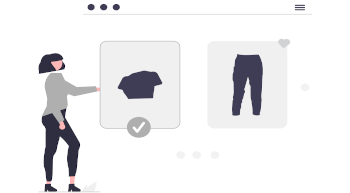
\includegraphics[width=0.8\linewidth]{web_shopping}
\captionof{figure}{Vente multi-plateforme}
\end{center}

Fashion-insta est un acteur majeur de la mode, en mettant à la porté de toutes, à des prix imbattables des articles dessinés par nos couturiers. Mais notre rôle de prescripteur de tendances, lequel nous galvanise pour nous dépasser, nous oblige à offrir la meilleure expérience pour nos clientes. Envoi chrono, retour sans frais, liste d’envies et surtout une recommandation d’articles à partir d’un selfie, dans son style.

\end{multicols}

%------------------------------------------------

\begin{multicols}{2}
\vspace{1em}

Notre méthode de vente s’appuie sur les usages des réseaux sociaux. Pour réaliser nos objectifs, nous nous appuyons sur la reconnaissance visuelle pour la recommandation d’articles, mais aussi sur une IA recomposant la photographie de la personne avec les articles que nous lui proposons. C’est un peu comme une expérience de mannequina avec une IA comme photographe, créative et originale. C’est pour cette fonctionnalité, que nous ouvrons le capital de l’entreprise à tous les investisseurs intéressés.


\begin{center}

\includegraphics[width=0.8\linewidth]{shooting}
\captionof{figure}{Expérience digitale nomade}
\end{center}

\end{multicols}
}

%----------------------------------------------------------------------------------------
%	REFERENCES
%----------------------------------------------------------------------------------------

\headerbox{References}{name=references,column=0,above=bottom}{

\renewcommand{\section}[2]{\vskip 0.05em} % Get rid of the default "References" section title
\nocite{*} % Insert publications even if they are not cited in the poster
\small{ % Reduce the font size in this block
\bibliographystyle{unsrt}
\bibliography{sample} % Use sample.bib as the bibliography file
}}

%----------------------------------------------------------------------------------------
%	Recherche Future
%----------------------------------------------------------------------------------------

\headerbox{Recherche Future}{name=futureresearch,column=1,span=2,aligned=references,above=bottom}{ % This block is as tall as the references block

\begin{multicols}{2}
Une intégration des dernières technologies en matière d’IA et d’UX représente une expression claire de nos objectifs de recherches futures.

Le compromis entre économie d’énergie, éthique et le besoin de nos clientes guide nos pas, pour devenir les leader du marché européen.
\end{multicols}
}

%----------------------------------------------------------------------------------------
%	CONTACT INFORMATION
%----------------------------------------------------------------------------------------

\headerbox{Contact Information}{name=contact,column=3,aligned=references,above=bottom}{ % This block is as tall as the references block

\begin{description}\compresslist
\item[Web] blog.rboyrie.info
\item[Email] romain@boyrie.email
\item[Phone] +33 6 72 09 32 31
\end{description}
}

%----------------------------------------------------------------------------------------
%	CONCLUSION
%----------------------------------------------------------------------------------------

\headerbox{Conclusion}{name=conclusion,column=2,span=2,row=0,below=results,above=references}{

\begin{multicols}{2}

\tikzstyle{decision} = [diamond, draw, fill=blue!20, text width=4.5em, text badly centered, node distance=2cm, inner sep=0pt]
\tikzstyle{block} = [rectangle, draw, fill=blue!20, text width=5em, text centered, rounded corners, minimum height=4em]
\tikzstyle{line} = [draw, -latex']
\tikzstyle{cloud} = [draw, ellipse, fill=red!20, node distance=3cm, minimum height=2em]

\begin{tikzpicture}[node distance = 2cm, auto]
\node [block] (init) {COMEX \\ V1};
\node [cloud, left of=init] (Start) {Fashion-Insta};
\node [cloud, right of=init] (Start2) {Investors};
\node [block, below of=init] (init2) {Release \\ V2};
\node [decision, below of=init2] (End) {Huge \\ Profits};
\path [line] (init) -- (init2);
\path [line] (init2) -- (End);
\path [line, dashed] (Start) -- (init);
\%path [line, dashed] (Start2) -- (init);
\path [line, dashed] (Start2) |- (init2);
\end{tikzpicture}

%------------------------------------------------

\begin{itemize}\compresslist
\item Nos jeunes clientes ont un mode de vie acceptant les nouvelles technologies du numérique. Notre devoir est de leur donner la meilleure expérience d’achat.
\item Nos recherches nous ont portés sur une IA capable de conseiller les clientes.
\item Nos équipes de marketing ont mis les clients au centre de l’application pour que les investisseurs puissent nous suivre dans cette formidable aventure.
\item Plus qu’une application, c’est la recommandation d’articles à partir d’un selfie de la personne avec une chaîne logistique permettant un achat fluide et sans contrainte, pour nos clientes.
\end{itemize}

\end{multicols}
}

%----------------------------------------------------------------------------------------
%	MATERIALS AND METHODS
%----------------------------------------------------------------------------------------

\headerbox{Méthodes Marketing}{name=method,column=0,below=objectives,bottomaligned=conclusion}{ % This block's bottom aligns with the bottom of the conclusion block

Les éléments suivants étaient requis pour notre application:

\begin{itemize}\compresslist
\item Le budget de départ
\item Un processus incluant le client
\item Une optimisation des ressources
\item Une estimation des revenus
\end{itemize}

L’équation suivante a été utilisé pour le ROI :

\begin{equation}
x^{\frac{\alpha-1}{\alpha}} \times y^{1/\alpha} \times \beta
\label{eq:revenu}
\end{equation}

Nous sommes déterminer à réaliser un profit, avec une prise de risque échelonnée à une dimension raisonnable, comportant autant de palier que nécessaire. En effet notre méthode préconise un mode SCRUM, lequel réalise idéalement des retours d’expérience client, avant la production à grande échelle.

Nous avons trouvé, par l’équation ci-dessus, la taille de l’équipe et le nombre de serveurs pour obtenir un ROI de 30\% par rapport aux capitaux engagés par notre pôle financier. Nous avons choisi d’accepter les investisseurs pour nous permettre de prendre plus de part de marché.

}

%----------------------------------------------------------------------------------------
%	RESULTS 2
%----------------------------------------------------------------------------------------

\headerbox{Usage des fonds}{name=results2,column=1,below=objectives,bottomaligned=conclusion}{ % This block's bottom aligns with the bottom of the conclusion block


Les données d’évaluation de l’usage des fonds et de leur impact sont présentées ci-dessous. Nos mécènes ont financé une première version.

\begin{center}
\begin{tabular}{l l l}
\toprule
\textbf{Service} & \textbf{\% Invest} & \textbf{\% ROI}\\
\midrule
Code & 40 & 15 \\
Serveur & 15 & 15 \\
Data & 45 & 70 \\
\bottomrule
\end{tabular}
\captionof{table}{Perte \& Profit matériels}
\end{center}

Nous souhaitons porter cette expérience loin. Nos équipes de recherche en IA garantissent des résultats spectaculaires dans très peu de temps. Mais nous anticipons une forte demande, compte-tenu de la qualité de ce placement.

\begin{center}
\begin{tabular}{l l l}
\toprule
\textbf{Service} & \textbf{\% Invest} & \textbf{\% ROI}\\
\midrule
Marketing & 35 & 20 \\
Ingénieur & 25 & 30 \\
Chercheur & 40 & 50 \\
\bottomrule
\end{tabular}
\captionof{table}{Perte \& Profit RH}
\end{center}
}

%----------------------------------------------------------------------------------------

\end{poster}

\end{document}